\documentclass[french]{msereport}

\usepackage{minted}

\newcommand{\gae}{\brand{Google App Engine}}

\title{PaaS - Google App Engine}
\module{CLOUD}{Cloud Computing}
\author{Jonathan Cornaz}

\begin{document}
	
	\section{Introduction}
		% TODO

	\subtitledsection[Exercice 1]{Déploiement d'une simple application web}
		L'exemple généré est un simple "Hello world". Il est constitué de trois fichiers clés : \code{index.html}, \code{web.xml} et \code{Lab04Servlet.java}.
		
		\subsection{Fichier index.html}
			A la racine de l'application apparaît un fichier \code{index.html} qui contient une redirection vers l'url "/Labo04".
		
		\subsection{Fichier web.xml}
			Le fichier de description d'application web (\code{web.xml}) résoud l'url "/Labo4" pour démarrer l'applet java en fonction de son nom de classe (en l'occurence "ch.hesso.mse.cloud.Lab04Servlet")
		
		\subsection{Fichier *.java}
			Le servlet (\code{Lab04Servlet.java}) est une classe dérivée de \code{HttpServlet} et implémente une méthode {doGet(HttpServletRequest, HttpServletResponse)}. En l'occurence l'implémentation consiste en la déclaration d'un contenu text et de l'impression du message "Hello world".
			
	\subtitledsection[Exercice 2]{Développer un \eng{Servlet} qui utilise le \eng{datastore}}
		\inputminted[
				frame=lines,
				fontsize=\footnotesize,
				linenos,
				label=Code du servlet,
				firstline=17
			]
			{java}
			{../Lab04/src/ch/hesso/mse/cloud/DatastoreWrite.java}
			
		\begin{figure}[h]
			\label{ds_viewer_local}
			\centering
			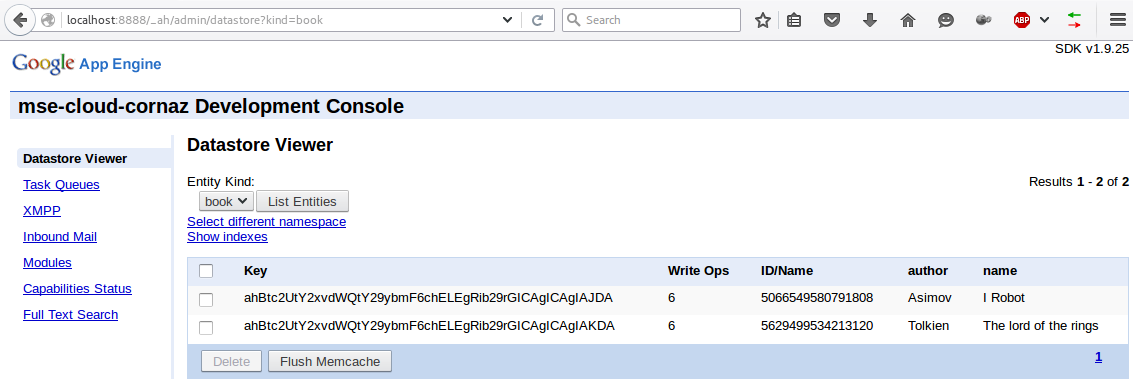
\includegraphics[width=\textwidth]{screen_ds_viewer_local.png}
			\caption{Résultat dans le Datastore viewer en local}
		\end{figure}
				
		\begin{figure}
			\label{ds_viewer_cloud}
			\centering
			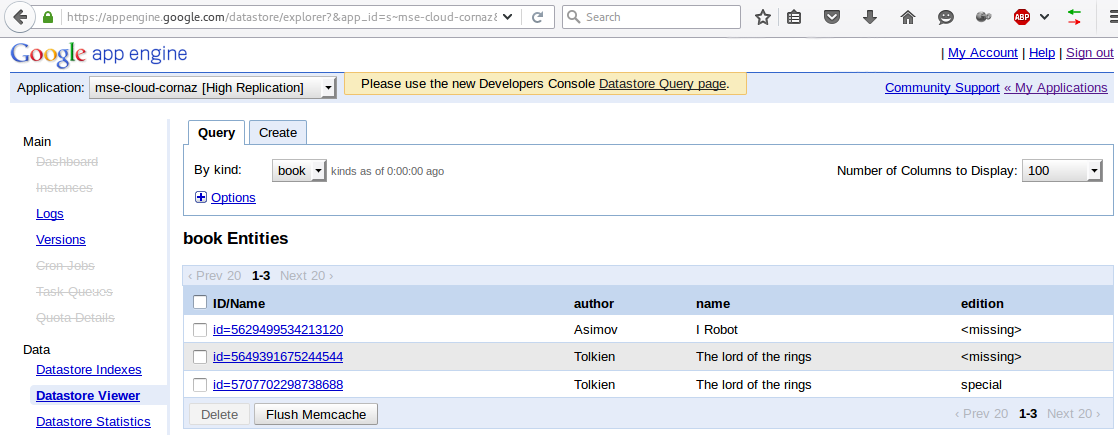
\includegraphics[width=\textwidth]{screen_ds_viewer_cloud.png}
			\caption{Résultat dans le Datastore viewer du cloud}
		\end{figure}
	
	\appendixsection
		
		\listoffigures
\end{document}
